\documentclass[twoside]{article}

\usepackage{ucs}
\usepackage[utf8x]{inputenc}
\usepackage{graphicx}
\usepackage{nopageno}
\usepackage{textcomp}

% ------
% Fonts and typesetting settings
\usepackage[sc]{mathpazo}
\usepackage[T1]{fontenc}
\linespread{1.05} % Palatino needs more space between lines
\usepackage{microtype}
\usepackage{ngerman}

% ------
% Page layout
\usepackage[hmarginratio=1:1,top=32mm,columnsep=20pt]{geometry}
\usepackage[font=it]{caption}
\usepackage{paralist}
\usepackage{multicol}

% ------
% Lettrines
\usepackage{lettrine}


% ------
% Abstract
\usepackage{abstract}
	\renewcommand{\abstractnamefont}{\normalfont\bfseries}
	\renewcommand{\abstracttextfont}{\normalfont\small\itshape}


% ------
% Titling (section/subsection)
\usepackage{titlesec}
\titleformat{\section}[block]{\large\scshape\centering{\thesection.}}{}{1em}{}
\titleformat{\subsection}[block]{\large\scshape\centering{\thesubsection}}{}{1em}{}


% ------
% Header/footer
\usepackage{fancyhdr}
	\pagestyle{fancy}
	\fancyhead{}
	\fancyfoot{}
	\fancyhead[C]{Einreichung zu TdSE 2015 $\bullet$ Industrievortrag $\bullet$ Jastram, Dorka}
	\fancyfoot[RO,LE]{\thepage}


% ------
% Clickable URLs (optional)
\usepackage{hyperref}

% PDF Metadata
\hypersetup{
    unicode=true,          % non-Latin characters in Acrobat’s bookmarks
    pdftoolbar=true,        % show Acrobat’s toolbar?
    pdfmenubar=true,        % show Acrobat’s menu?
    pdffitwindow=true,     % window fit to page when opened
    pdfstartview={FitH},    % fits the width of the page to the window
    pdftitle={Einreichung zur TdSE 2015: Solide Anforderungen dank ReqIF im europäischen Schienenverkehr},    % title
    pdfauthor={Michael Jastram, Moritz Dorka},     % author
    pdfsubject={Industrievortrag},   % subject of the document
    pdfnewwindow=true,      % links in new window
    colorlinks=true,       % false: boxed links; true: colored links
    linkcolor=blue,          % color of internal links
    citecolor=blue,        % color of links to bibliography
    filecolor=blue,      % color of file links
    urlcolor=blue           % color of external links
}

% ------
% Maketitle metadata
\title{\vspace{-15mm}%
	\fontsize{24pt}{10pt}\selectfont
	\textbf{Solide Anforderungen dank ReqIF im europäischen Schienenverkehr}
	}	
\author{%
	\large
	\textsc{Michael Jastram, Moritz Dorka} \\[2mm]
	\normalsize	Formal Mind GmbH \\
	\normalsize	TU Dresden
	\vspace{-5mm}
	}
\date{}

%\usepackage[left=2cm,top=0.9cm,right=2cm,bottom=3cm,nohead,nofoot]{geometry}
%\titleformat{\section}{\large\bfseries}{\thesection}{compact}{}


%%%%%%%%%%%%%%%%%%%%%%%%
\begin{document}

\maketitle
\thispagestyle{fancy}

\begin{abstract}
\noindent Im Zug von Düsseldorf über Brüssel nach Paris – das ist heute schon möglich, dank ETCS, dem European Train Control System.  Diese Spezifikation beschreibt die Kommunikation zwischen Signalanlagen und Zug. Leider wurde bei der Erstellung im Jahre 1998 auf den kleinsten gemeinsamen Nenner zurückgegriffen, MS Word. Das Ergebnis sind tausende Seiten, die schwer zu pflegen und inkonsistent formatiert und über viele Dateien verteilt sind.  Im Rahmen des ITEA-Projekts openETCS wurde ein Konverter entwickelt, mit dem diese Dokumente in das offene, international standardisierte ReqIF überführt werden kann.  Das ReqIF-basierte Anforderungsmodell wird dann im Projekt als Basis für die weitere Systemmodelllierung eingesetzt, wo es von verschiedenen Werkzeugen konsumiert werden kann.
\end{abstract}
	
\begin{multicols}{2}
\noindent 

%=========================================================================
\section{Einleitung}
% 1 Seite, zum Schluss schreiben
%=========================================================================

Grenzüberschreitender Bahnverkehr klingt so einfach! Autos und Flugzeuge überqueren zwar schon lange regelmäßig Grenzen, aber im Schienenverkehr ist das noch nicht lange möglich.  Die Probleme der Hardware wurden längst gelöst, also Themen wie Spurweite und Oberleitungen.  Das Hauptproblem sind die hohen Sicherheitsanforderungen im Schienenverkehr, die nur gewährleistet werden können, wenn die Signalanlagen einheitlich aufgebaut sind und konsistent funktionieren.  Die bestehenden Systeme zu vereinheitlichen kam gar nicht in Frage -- allein die Vereinheitlichung der deutschen Signalanlagen nach der Wiedervereinigung hatte 20 Jahre gedauert!  Daher wurde ein neuer Standard geschaffen, das Europen Train Control System (ETCS).

Doch der Weg dorthin war holprig, nicht zuletzt, weil der ETCS-Ansatz sich erheblich von konventionellen Systemen unterscheidet.  Insbesondere wird ein zunehmender Teil der der Sicher­heitsfunktionen, die bisher durch die Stre­ckeneinrichtungen wahrgenommen worden sind, in das Fahrzeuggerät verlagert, was die Komplexität der Steuergeräte erheblich erhöht \cite{Hase2011}.  Das kann vorteilhaft für die Netzbetreiber sein, erhöht aber die Kosten der Fahrzeuge.  Laut einer Studie der DB würde es über 230~T€ pro Triebkopf kosten, ICEs mit ETCS auszustatten - die Kosten für konventionelle Technologie liegt bei ca. 60~T€, also ca. einem Viertel \cite{Hase2009}.

Nicht nur die Komplexität erhöht die Kosten, auch die Form der Spezifikation, denn diese besteht aus hunderten von in Word geschriebenen Seiten (siehe \ref{sec:subset-26}).  Zum einen ist die Wartung dieser Dokumente ein Alptraum, der sich in vielen Kapiteln mit der Überschrift \glqq{}Intentionally Deleted\grqq{} manifestiert. Weiterhin werden tief verschachtelte Kapitelnummerierungen als IDs benutzt, zum Beispiel für Querverweise.  Manche Querverweise nutzen die Funktionalität von Word, aber manchmal wurde einfach die entsprechende Nummer händisch hineingeschrieben.  Kein Wunder, dass die Produkte unterschiedlicher Hersteller im Markt nicht hundertprozentig kompatibel sind.

%-------------------------------------------------------------------------
\subsection{openETCS}
\label{sec:openetcs}
% 1 Seite, Michael
%-------------------------------------------------------------------------

Das openETCS ist ein itea Forschungsprojekt, welches Ende 2015 abgeschlossen wird \cite{itea-openetcs}. Es wurde primär geschaffen, um die Kosten zu senken und Kompatibilität zu erhöhen.  Das Mittel dazu sollte \glqq{}Open Proofs\grqq{} sein:  Damit ist gemeint, dass zentrale Artefakte für alle interessierten offen zugänglich sein sollen, offenen Standards für die Speicherung nutzen, und mit offenen Werkzeugen bearbeitet werden können.  Die Idee ist, dass die Beschreibung von ETCS keinen Wettbewerbvorteil bietet, daher liegt es im Interesse von Wettbewerbern, auf dieser Ebene zusammenzuarbeiten.  Einzelne Firmen wie Alstom, Thales oder Siemens können sich dann durch ihre konkrete Implementierungen (also den eigentlichen Steuergeräten) im Markt differenzieren.  Dadurch, dass die verschiedenen Geräte auf dem selben Systemmodell aufsetzen, soll sich auch die Kompatibilität verbessern.

Der Scope von openETCS beschränkt sich auf die Modellierung der Software.  Für die Modellierung auf Systemebene wurde SysML ausgewählt, für das Eclipse Papyrus als offenes Werkzeug zur Verfügung steht.  Die eigentlichen Anforderung lagen jedoch als Berg von Word-Dokumenten vor.  Die in der Bahnindustrie relevanten Standards (insbesondere EN50128) erforndern eine saubere Nachverfolgbarkeit.  Da diese mit Word nicht möglich ist, mussten die Dokumente erst einmal entsprechend aufbereitet werden. Dies konnte mit Hilfe des ReqIF-Standards und des offenen Eclipse Requirements Modeling Frameworks erfolgreich realisiert werden.

%-------------------------------------------------------------------------
\subsection{Subset-026}
\label{sec:subset-26}
% ½ Seite, Moritz
%-------------------------------------------------------------------------

ETCS besteht aus diversen Teilsystemen, deren jeweilige Spezifikationen unabhängig voneinander gepflegt werden. Die Kernfunktionalität des Systems wird in dem gut 500-seitigen Dokument \glqq{}Subset-026\grqq{} beschrieben, das wiederum aus acht, in einzelnen Dateien verwalteten Kapiteln besteht.

Thematisch behandelt das \glqq{}Subset-026\grqq{} hauptsächlich einen Fahrzeugrechner, den sogenannten European Vital Computer (EVC) und dessen Schnittstellen. Der EVC kommuniziert über drei verschiedene Arten (punktförmiger Transponder, Leiterschleife und Funk) mit den streckenseitigen Einrichtungen und verfügt zudem über eine Mensch-Maschine-Schnittstelle (Driver Machine Interface) über die der Triebfahrzeugführer Eingaben vornehmen kann. All diese Daten verarbeitet der Rechner kontinuierlich und leitet daraus Aktionen für das Fahrzeug ab (Bremsen, Beschleunigen, Stromabnehmer heben/senken, \ldots ).

Neben dem \glqq{}Subset-026\grqq{} gibt es zahlreiche weitere Subsets, die sich mit den vom EVC angesteuerten Komponenten befassen. Deren breit gefächerte Inhalte reichen von funktionalen Anforderungen an eine fahrzeugseitige Aufzeichnungseinheit (eine Art \glqq{}Black-Box\grqq{}) über streckenseitige Stellwerksschnittstellen bis hin zu kryptographischen Details für die Funkverbindung. Alle Spezifikationen werden von der European Railway Agency, einer EU-Behörde, zentral verwaltet und sind als Word- und PDF-Dokumente verfügbar.

Doch hier ergibt sich ein weiteres Problem: Die Anforderungen von Subset-026 haben leider keine IDs: Stattdessen wurden die von Word generierte Listennummerierung für die Identifizierung von Anforderungen herangezogen. Leider wurde diese nicht konsistent angewendet, wodurch Querverweise teilweise als einfacher Text eingefügt wurden, und viele Überschriften den Titel \glqq{}Intentionally Deleted\grqq{}, oder ähnliches, enthalten.

%-------------------------------------------------------------------------
\subsection{ReqIF}
% ½ Seite, Michael
%-------------------------------------------------------------------------

Auch wenn die Nachverfolgbarkeit von Subset-026 manuell über diese Listennummerierung realisiert werden könnte, ist dies kein empfehlenswertes vorgehen (gelinde ausgedrückt!).  Daher wurde entschieden, das Subset-026 in das Requirements Interchange Format (ReqIF) zu überführen. 

ReqIF \cite{openup} ist ein internationaler Standard zum Austausch von Anforderungen, der von der OMG herausgegeben wird.  Viele verbreitete Anforderungs-Werkzeuge wie IBM DOORS, PTC Integrity oder Polarion ALM ermöglichen inzwischen den Anforderungsaustausch per ReqIF.  Damit hat ReqIF die vom Open Proofs-Ansatz geforderten Eigenschaften.  Und nicht nur das: Mit dem Eclipse Requirements Modeling Framework (RMF) gibt es bereits eine quelloffnene Referenzimplementierung, um mit ReqIF-Daten umzugehen. Wie in \ref{sec:openetcs} beschrieben, wurde die Entscheidung gefällt, die Systemmodellierung mit Eclipse Papyrus durchzuführen.  Durch die gemeinsame Technologieplattform Eclipse ist damit auch eine Integration leicht realisierbar, was in \ref{sec:traceability} noch weiter erörtert wird.

Das ReqIF-Format ermöglicht es, alle wichtigen Strukturen eines Anforderungsmodells abzubilden.  Dabei benutzt ReqIF eine eigenwillige Terminologie.  Anforderungen werden SpecObjects genannt und können typisiert werden.  Der Typ bestimmt dann, welche Attribute die Anforderung hat, bspw. Anforderungstext, ID, Status, Autor, etc. Die einzelnen Attribute sind ebenfalls typisiert, zum Beispiel als Text, Zahl, Aufzählung, formatierter Text (XHTML), etc.

Anforderungen können in Sichten zusammengefasst werden, wodurch ein hierarchisches Anforderungsdokument, die Specification, entsteht.  Weiterhin können Anforderungen untereinander über SpecRelations verlinkt werden. Auch Specifications und SpecRelations können Typen und Attribute haben.

ReqIF hat noch viele weitere Eigenschaften, auf die wir hier nicht weiter eingehen wollen, und die im Detail in der ReqIF Spezifikation \cite{reqif} beschrieben sind.

%=========================================================================
\section{Von Word nach ReqIF}
%=========================================================================

Bevor wir uns mit der eigentlichen Konvertierung der Anforderungen von Word nach ReqIF beschäftigen, wollen wir erläutern, wie genau die Anforderungen in der Entwicklung eingesetzt werden sollen.

%-------------------------------------------------------------------------
\subsection{Anforderungen im V-Modell}
% ½ Seite, Michael
%-------------------------------------------------------------------------

Im Schienenbereich bewegen wir uns im sicherheitskritischen Bereich, wo entsprechende Vorschriften herrschen.  Maßgeblich ist hier EN 50128 \cite{en50128}, eine Spezialisierung der EN 61508 für sicherheitsrelevante Software der Eisenbahn.  Hardware ist nicht im Scope von openETCS.  Der im Standard beschriebene Entwicklungsprozess orientiert sich am V-Modell, welches dort auch beschrieben ist (Figure~\ref{fig:v-modell}). 

\begin{figure*}
\centering
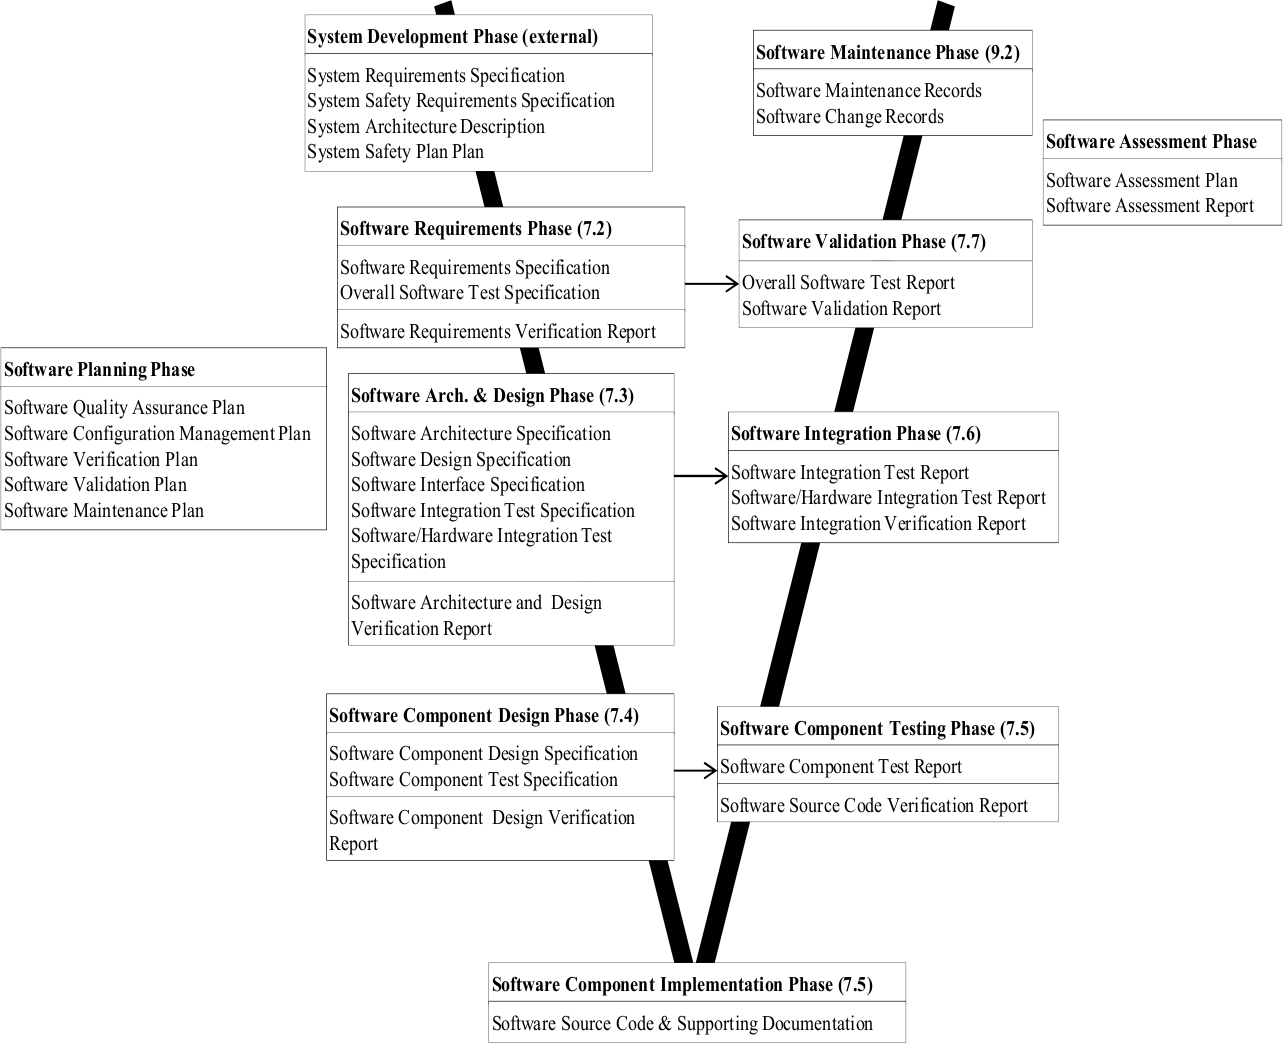
\includegraphics[width=0.8\linewidth]{img/v-modell.png}
\caption{{Das V-Modell aus \cite{en50128}, Seite 23, Abb. 4}}
\label{fig:v-modell}
\end{figure*}

Das V-Modell zeichnet sich unter anderem dadurch aus, dass Anforderungen und deren Verfolgbarkeit eine zentrale Rolle spielen: Anforderungen bilden den Ausgangspunkt der Entwicklung (\glqq{}links oben\grqq{}), wovon sich nachfolgend Artefakte bis zur Implementierung ableiten (\glqq{}Mitte unten\grqq{}). Wie viele Zwischenschritte es gibt, hängt von der Größe der Entwicklung ab.  Gleichzeitig gibt es eine \glqq{}horizontale\grqq{} Nachverfolgbarkeit (Traceability) zu den entsprechenden Tests auf den verschiedenen Ebenen (\glqq{}rechter Ast\grqq{}).

%-------------------------------------------------------------------------
\subsection{Traceability von Anforderungen}
\label{sec:traceability}
% ½ Seite, Michael
%-------------------------------------------------------------------------

Ziel des openETCS-Projekts ist es, mit offenen Standards und offenen Werkzeugen die Entwicklung durchzuführen.  Dabei wurden verschiedene Ansätze, Werkzeuge und Technologien evaluiert.  Insbesondere wurde das auf Eclipse basierende PolarSys-Werkzeug \cite{polarsys} in Betracht gezogen.  Letzten Endes wurde nur eine Komponente von PolarSys für openETCS ausgewählt, und zwar Eclipse Papyrus \cite{papyrus}.  Papyrus ist ein Werkzeug für die UML- und SysML-Modellierung.  Für die Anforderungen wurden dementsprechend SysML-Requirements in Betracht gezogen, aber wieder verworfen: Zum einen skaliert Papyrus bei weitem nicht gut genug um die zahlreichen im Subset-026 enthaltenen Anforderungen zu verwalten.  Zum anderen sollte die Traceability direkt in den ursprünglichen Text des Subset-026 möglich sein.

Um dennoch eine Traceability zwischen den Anforderungen des Subset-026 (als ReqIF) und dem SysML-Modell (Papyrus) zu ermöglichen, wurden ebenfalls mehrere Ansätze evaluiert.  Zum einen wurde im Projekt ein Traceability-Plug-in entwickelt, welches die Verlinkung über Drag\&Drop ermöglicht, und die Verlinkung in ReqIF-SpecRelations abspeichert \cite{rmf-traces}.  Attraktiv bei diesem Ansatz ist, dass die Verlinkung im ReqIF-Modell liegt, und damit auch anderen Werkzeugen zugänglich gemacht werden kann (bspw. durch einen Import nach IBM DOORS).

Da die Traceability jedoch auch über das SysML-Modell hinausgehen und auch für Daten zugänglich sein soll, die nicht im Eclipse-Ökosystem liegen, wurden zwei weitere Ansätze identifiziert.  Zum einen wurde Eclipse ReqCycle \cite{Todo} als generische Traceability-Lösung in Betracht gezogen.  Allerdings ist es nicht ausgereift genug, um schon eingesetzt zu werden.  Weiterhin wird für Teile das proprietäre Reqtify eingesetzt.  Um eine durchgängige und zuverlässige Traceability zu ermöglichen, wurde bei der Konvertierung von Word besonders Wert auf die Erzeugung der IDs gelegt, wie in \ref{sec:ids} beschrieben ist.

%-------------------------------------------------------------------------
\subsection{Word: Herausforderungen}
% ½ Seite, Moritz
%-------------------------------------------------------------------------


\begin{figure*}
\centering
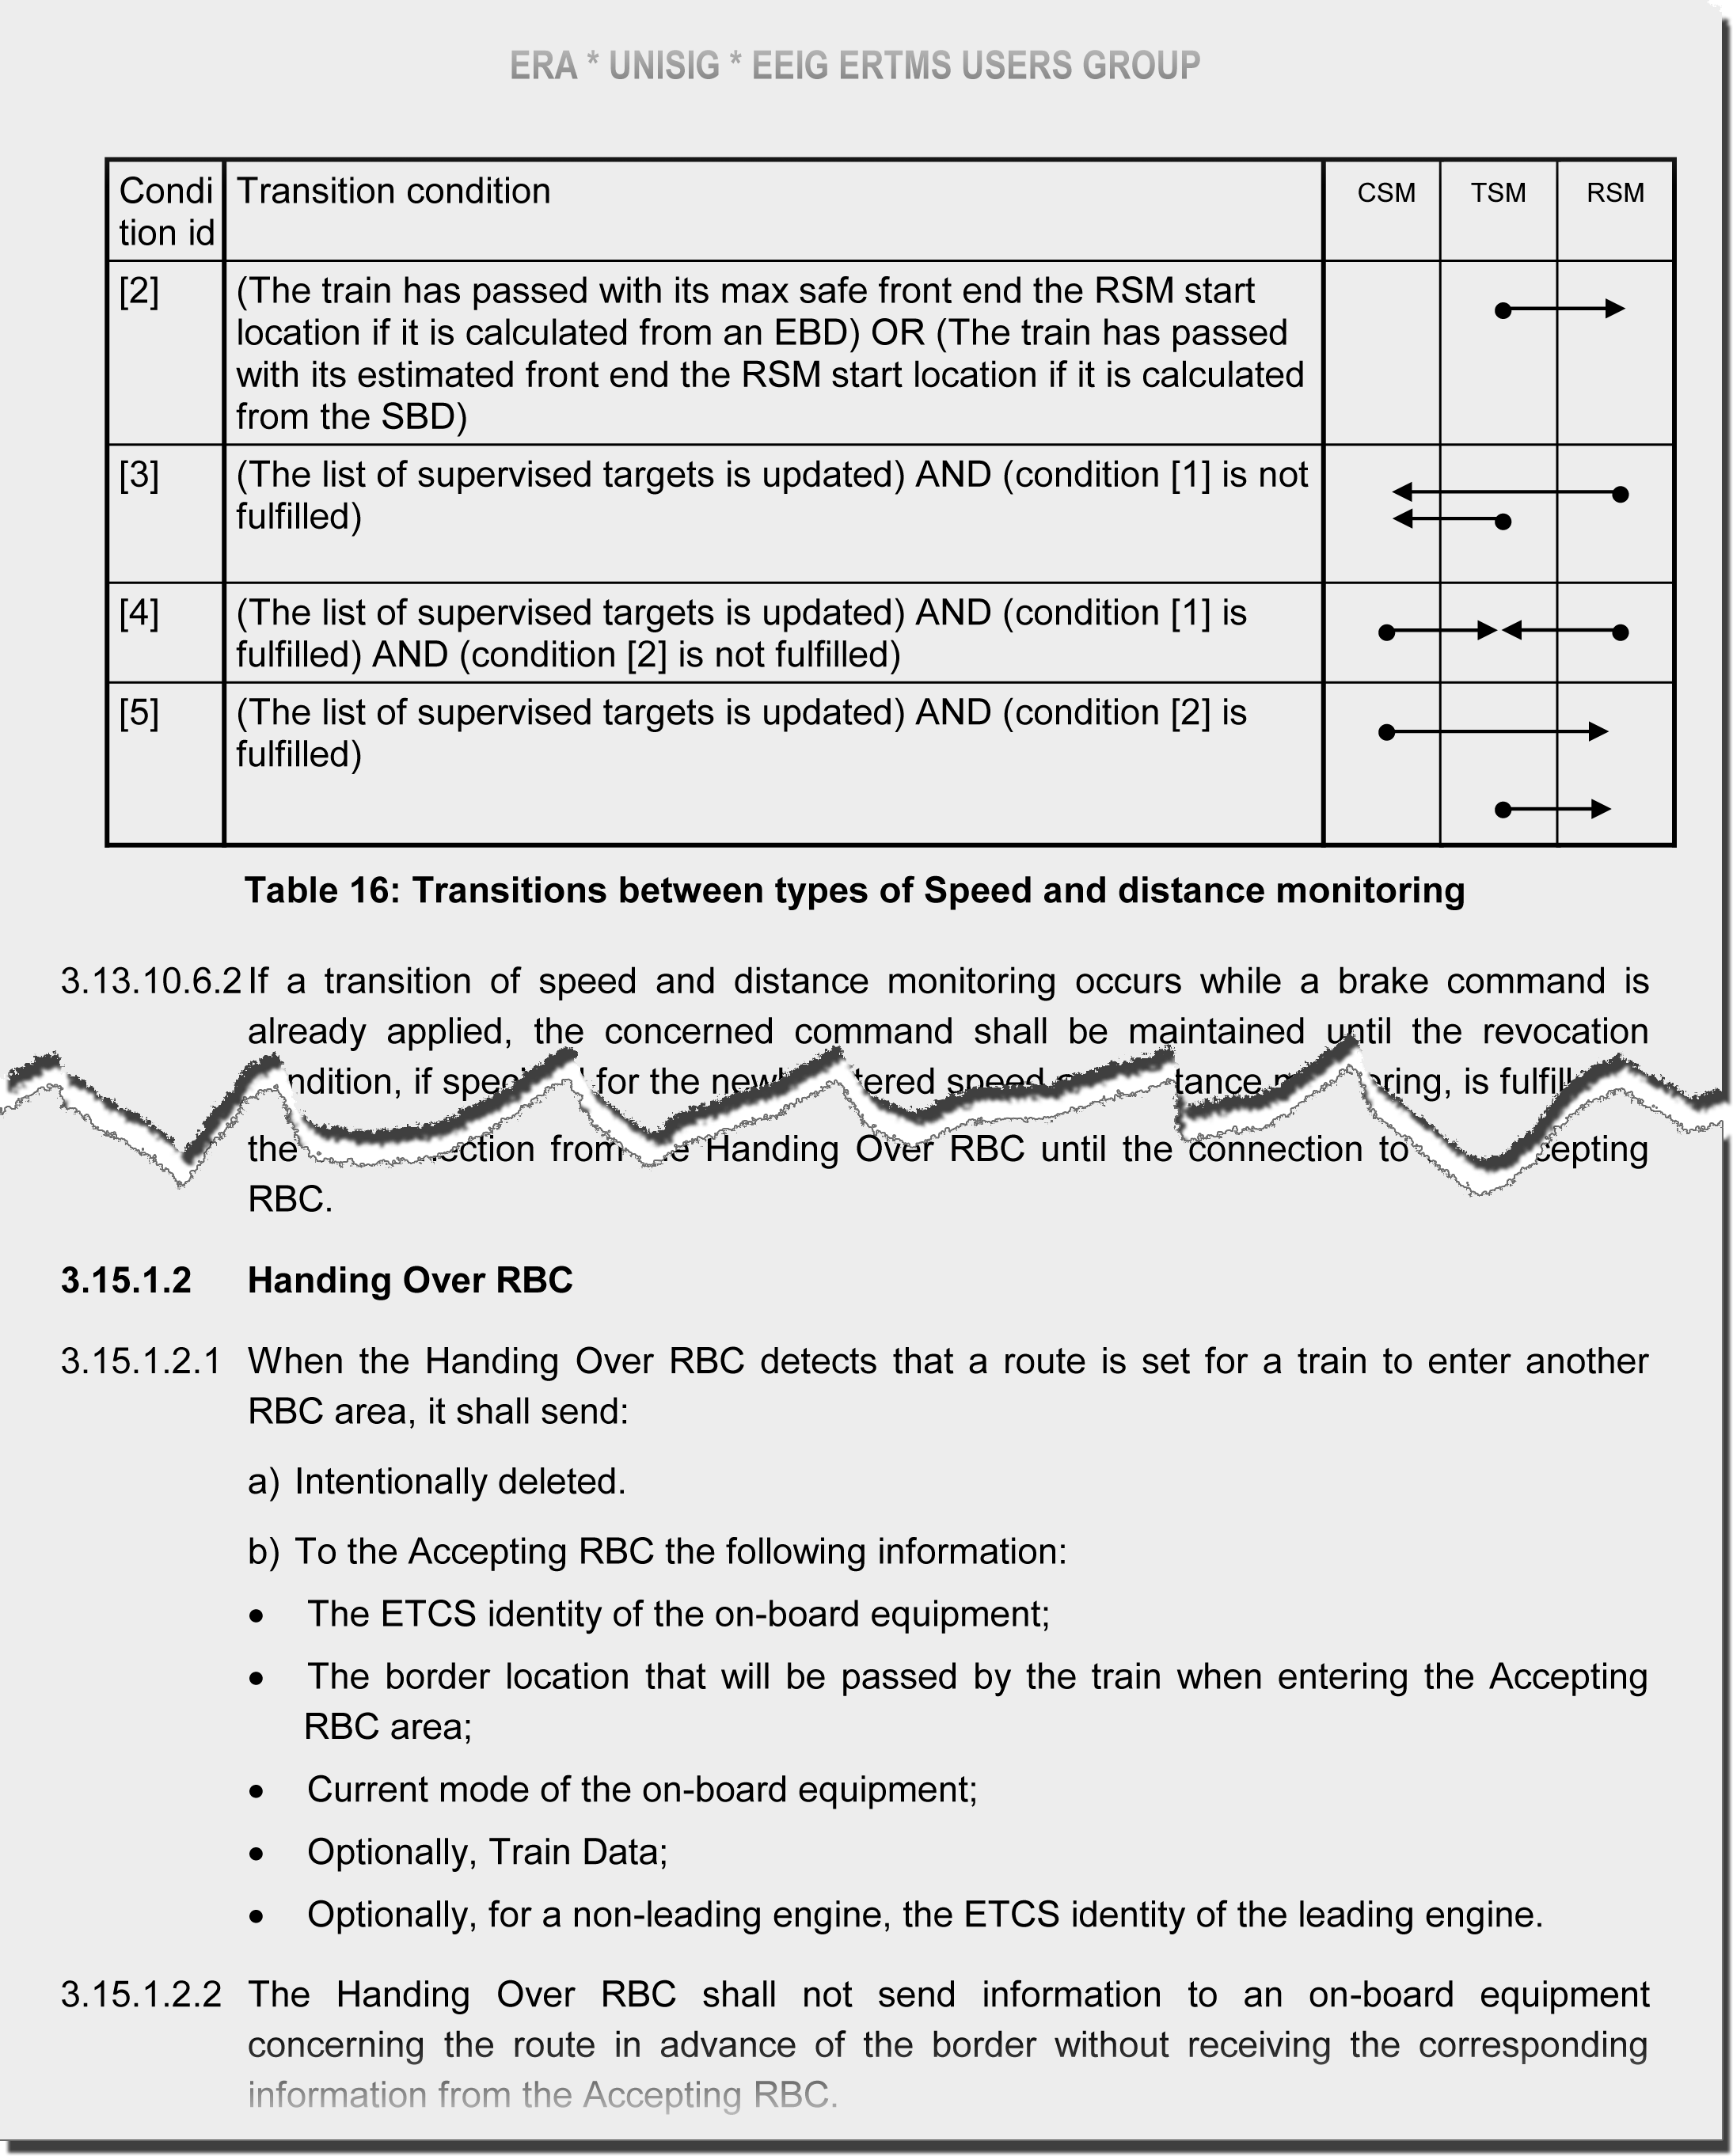
\includegraphics[width=0.8\linewidth]{img/word_screenshot.png}
\caption{Beispielhaftes Layout von chapter 3 des Subset-026}
\label{fig:word_screenshot}
\end{figure*}

Microsoft Word ist ein Textverarbeitungsprogramm für die breite Masse. Es versucht dementsprechend möglichst viele Anwendungsbereiche abzudecken und dem Nutzer dabei möglichst wenige Einschränkungen zu machen. Dies führt unweigerlich zu einer sehr komplexen Software (\glqq{} eierlegende Wollmilchsau\grqq{}) und spiegelt sich auch in dem zugrundeliegenden Dateiformat wider. Zudem verführt die Verfügbarkeit all dieser Funktionen den Nutzer bisweilen auch zu deren Verwendung -- was insbesondere im Umfeld von technischen Dokumentationen nicht unbedingt vorteilhaft sein muss.

Das mit Abstand größte Manko an Word aus Sicht des Anforderungsmanagements ist allerdings das Fehlen einer klaren semantischen Struktur. Es ist also nicht in jedem Fall ohne Weiteres möglich aus dem Fließtext eines solchen Dokuments einzelne, genau abgegrenzte Anforderungen zu extrahieren. Vielmehr sind hier domänenspezifische Algorithmen notwendig, die kontextabhängig sinnvolle, möglichst atomare Elemente in dem Datenstrom des Worddokuments erkennen und ihnen eindeutige Bezeichner für die spätere Traceability zuweisen können. Ebenso muss eine algorithmenbasierte Formalisierung der diversen Formatierungen erfolgen. Durch die Unterstützung von XHTML bietet ReqIF zwar die Voraussetzungen um zahlreiche einfachere Auszeichnungen (Fettdruck, Unterstreichungen, \ldots{}) direkt zu übernehmen. Aber insbesondere bei stark layoutabhängigen Elementen (z.B. Pfeilen, vgl. Abbildung \ref{fig:word_screenshot} oben) hat sich die vorherige Umwandlung in eine Textform als sinnvoll erwiesen.

%-------------------------------------------------------------------------
\subsection{Lösungsansatz und Implementierung}
% 1 Seite, Moritz
%-------------------------------------------------------------------------


\begin{figure*}
\centering
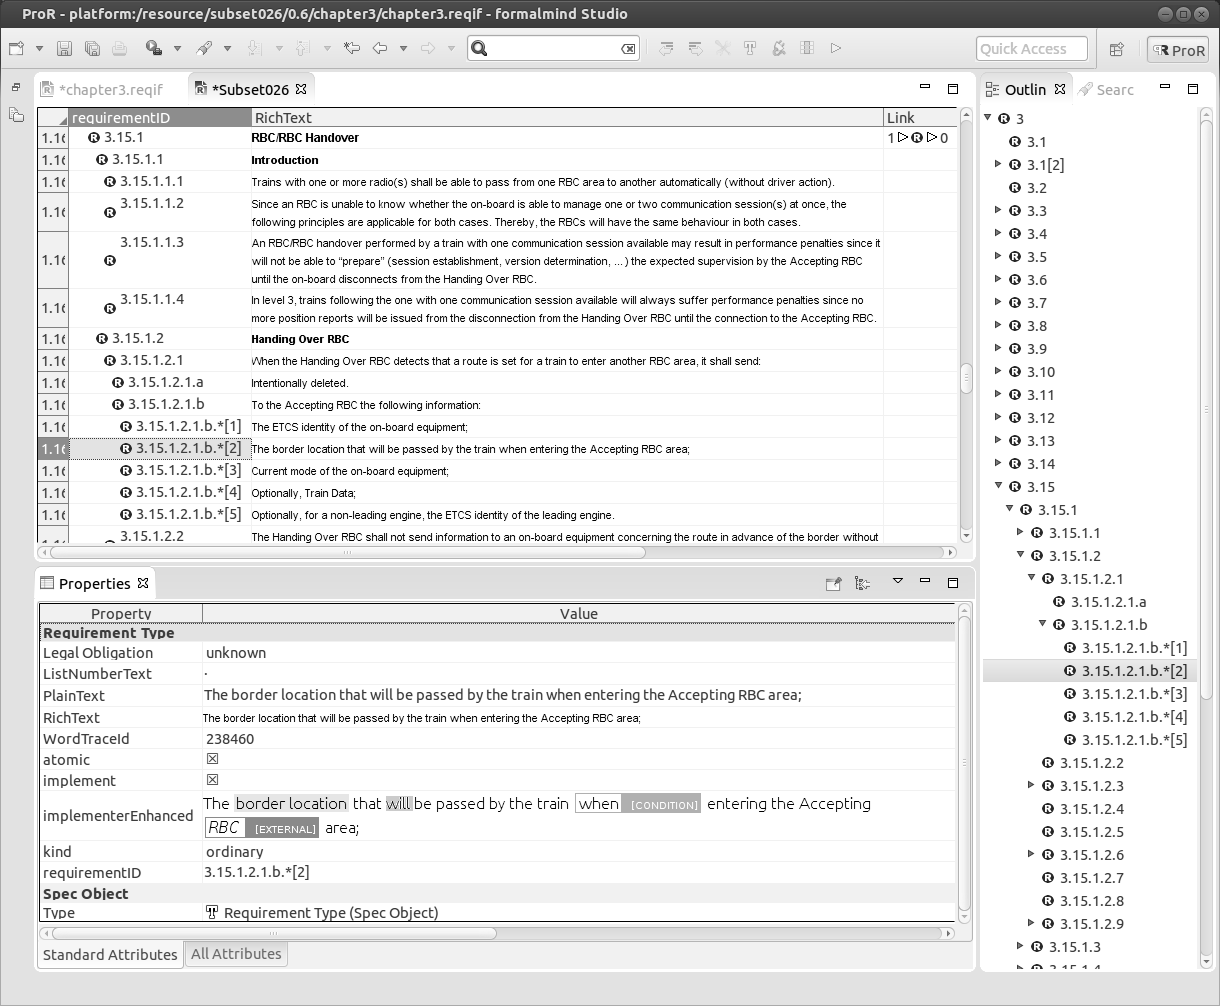
\includegraphics[width=0.8\linewidth]{img/pror_screenshot.png}
\caption{Darstellung des unteren Teils von Abbildung \ref{fig:word_screenshot} in ProR}
\label{fig:pror_screenshot}
\end{figure*}

Vorhandene Werkzeuge zum Import von Word-Spezifikationsdokumenten, wie sie beispielsweise in DOORS und reqtify/SCADE integriert sind, stellen gewisse Anforderungen an deren strukturellen Aufbau. Im vorliegenden Fall war es aber weder gewünscht noch mit vertretbarem Aufwand möglich diese Struktur durch Veränderungen im Ausgangsdokument herbeizuführen. Ohne derartige Anpassungen sind die Importergebnisse dieser Tools allerdings kaum brauchbar da gewisse, vermeintlich unwesentliche Details wie Tabellenhintergründe oder Pfeile (siehe oben) schlicht unterschlagen werden und die willkürlich generierten Identifikatoren der extrahierten Anforderungen mit dem bisher (manuell) genutzten, listenbasierten Adressierungsschema nicht harmonieren. Zudem ist keines der am Markt verfügbaren Werkzeuge quelloffen, was dem erklärten Projektziel entgegensteht.

Als Alternative wurde eine neuartige Software speziell für das \glqq{}Subset-026\grqq{} geschaffen, die vorab auf dessen Besonderheiten hin konfiguriert werden kann \cite{TodoMoriz}. Danach ist sie imstande vollkommen autark eine Konvertierung zu ReqIF mitsamt einer Aufwertung der textuellen Inhalte durchzuführen. Das Tool wurde in Java entwickelt und fußt auf einer stark angepassten Version von Apache POI, einer quelloffenen Implementierung des binären Word-Dateiformats, um die Spezifikationen einzulesen. Anschließend kommen domänenspezifische Algorithmen zum Einsatz, die auf Grundlage der teilweise vorhandenen Listennummerierung (vgl. Abbildung \ref{fig:word_screenshot}) menschenlesbare Bezeichner für die einzelnen Anforderungen generieren und wiederkehrende Elemente (Tabellen, Gleichungen, boolesche Beziehungen, \ldots{}) erkennen.

Im folgenden Aufwertungsschritt finden zahlreiche reguläre Ausdrücke und in sehr begrenztem Maße auch Algorithmen aus dem Bereich des Natural Language Processing Anwendung. Deren Ausgabe mündet in diversen Metadaten, die an die einzelnen Anforderungen in der resultierenden ReqIF-Datei angehangen werden und diese beispielsweise kategorisieren (Note, Example, deleted, \ldots ) oder deren Implementierungsnotwendigkeit (verpflichtend, optional, unklar, \ldots ) kodieren. Zudem gibt es ein spezielles Feld in dem der Anforderungstext annotiert wird um domänenspezifische Phrasen (z.B. \glqq Lineside Electronic Unit\grqq ) oder schwache Wörter (\glqq{}immediately\grqq{}, \glqq{}if possible\grqq{}, \ldots{}) hervorzuheben. Unabhängig davon werden auch verschiedene Arten von Querverweisen automatisiert ausgelesen, formalisiert und schließlich in deren ReqIF-Pendant überführt. Durch einen speziellen Zeiger, der ebenfalls in den Metadaten enthalten ist, wird zudem die Rückverfolgbarkeit in das Ausgangsdokument sichergestellt. Damit ist es möglich jederzeit an die Stelle in dem Word-Dokument zu springen die die Ausgangsdaten einer bestimmten Anforderung enthält.

Falls die ReqIF-Ausgabe auch die Abbildungen, OLE-Objekte (z.B. Gleichungen) und Zeichnungen des Ausgangsdokuments enthalten soll, ist dafür eine anschließende externe Konvertierung notwendig, die weiterhin Microsoft Word voraussetzt. Das Tool enthält dafür spezielle Makros um auch diesen Arbeitsschritt weitgehend zu automatisieren.

% Bild eines Abschnitts der Orignalspezifikationen einfügen damit der Leser einen Eindruck bekommt was "Listennummerierung" und "Pfeile" bedeutet?

%-------------------------------------------------------------------------
\subsection{Eindeutige IDs}
\label{sec:ids}
% ½ Seite, Moritz, Michael
%-------------------------------------------------------------------------

Eine große Herausforderung war der Umgang mit IDs. Wie bereits erwähnt, setzen die Ursprungsdokumente des Subset-026 dafür die Word-eigene Listennummerierung ein. Leider sind aber nicht alle Absätze Teil einer Liste und haben entsprechend nicht immer auch eine Nummer. Außerdem soll es möglich sein mit neuen Versionen des Subset-026 arbeiten zu können, ohne eine bestehende Verlinkung verwerfen zu müssen. Das bedeutet, dass die IDs deterministisch und eindeutig generiert werden müssen, während sie sich trotzdem noch an der Absatznummerierung orientieren.  Keine leichte Aufgabe.
% Todo Beispiel Screenshot

%=========================================================================
\section{Die Zukunft von openETCS}
%=========================================================================

Das Projekt openETCS endet mit Jahresende.  Die Ergebnisse im Bereich Open Source sind leider etwas enttäuschend.  Ursprünglich bestand die Hoffnung, auf einer bestehenden Plattform wie PolarSys aufzusetzen.  Doch leider stellte sich PolarSys als wesentlich unausgereifter heraus als ursprünglich gedacht.  Letzen Endes sind an offenen Komponenten nur RMF (ReqIF Requirements) und Papyrus (SysML) übriggeblieben.  Der Rest der Entwicklung wird über das proprietäre Scade Suite umgesetzt.  Aber gerade deswegen ist der Word-Converter ein Lichtblick, der die Ergebnisse des Projekts drastisch aufwertet. Denn über ReqIF sind die Anforderungen von Subset-026 wesentlich leichter zu verwerten, und die geschickte ID-Generierung des Konverters ermöglicht es, die Brücke auch in eine proprietäre Umgebung (in diesem Fall Scade Suite) zu schlagen.

Im Bereich Modellierung wurde mit Scade der Grundstein für eine herstellerübergreifende Arbeit geschaffen.  Das ist an sich schon ein gutes Ergebnis.  

Und nicht zuletzt wurden im Projekt auch weitere Ansätze verfolgt, um sich in Folgeprojekten von proprietären Werkzeugen lösen zu können.  Besonders vielversprechend ist ein Ansatz, SysML-Modelle nach B zu übersetzen \cite{sysml2b}. 

%-------------------------------------------------------------------------
\subsection{ReqIF und RMF in der Systementwicklung}
% 1 Seite, Michael
%-------------------------------------------------------------------------

Es gibt weitere Projekte, die ReqIF für die Modellierung von Anforderungen in der Systementwicklung einsetzen \cite{reqifolution,ix,eclipse-teaching}.  Insbesondere wird das Eclipse RMF-Framework von mindestens drei kommerziellen Anbietern eingesetzt, und uns sind mehrere firmeninterne Projekte bekannt, die auf RMF aufsetzen.

Erwähnenswert ist hier das Projekt SE Teaching \cite{se-teaching}.  Hier ist es das Ziel, mit offenen Standards und Werkzeugen eine Grundlage für die Lehre des Systems Engineering zu legen.  In diesem Projekt wird mit einer minimalen, Eclipse-basierten Entwicklungsumgebung gearbeitet, bei der RMF für das Anforderungsmanagement herangezogen wird.

%-------------------------------------------------------------------------
\subsection{Verwertung}
% 1½ Seiten; Michael & Moritz
%-------------------------------------------------------------------------

Alle Ergebnisse von openETCS sind offen lizenziert und über die Projektwebseite zugänglich \cite{itea-openetcs}.  Es laufen auch Aktivitäten für eine Nachfolgeprojekt mit dem Ziel, die Ergebnisse weiterzuentwickeln und sich mittelfristig von proprietären Ansätzen zu lösen.  Zahlreiche Partner des Projekts planen bereits, die Ergebnisse des Projekts auch kommerziell zu verwerteten.

%=========================================================================
\section{Fazit}
% ½ Seite
%=========================================================================

Das openETCS-Projekt hatte ambitionierte Ziele, die Entwicklung von ETCS-System mit \glqq{}Open Proofs\grqq{} radikal zu verändern. Das war ein hochgestecktes Ziel, das zu großen Teilen erreicht wurde, leider nicht in allen.

Aber insbesondere im Bereich Anforderungsmanagement hat dieses Projekt dazu beigetragen, den offenen ReqIF-Standard auch als Datenmodell für große Entwicklungen zu validieren.  Das Arbeiten mit Anforderungen im Eclipse RMF-Editor ist ein Quantensprung, verglichen mit der Spezifikation in Word. Wir gehen davon aus, dass diese Arbeit den ReqIF-Standard im Eisenbahnumfeld salonfähig machen wird.

\end{multicols}

\titleformat{\section}[block]{\large\scshape\centering{}}{}{1em}{}

\bibliographystyle{alpha}
\bibliography{bibliography}


\end{document}

